

\documentclass[man]{apa6}
\usepackage{lmodern}
\usepackage{amssymb,amsmath}
\usepackage{ifxetex,ifluatex}
\usepackage{fixltx2e} % provides \textsubscript
\ifnum 0\ifxetex 1\fi\ifluatex 1\fi=0 % if pdftex
  \usepackage[T1]{fontenc}
  \usepackage[utf8]{inputenc}
\else % if luatex or xelatex
  \ifxetex
    \usepackage{mathspec}
  \else
    \usepackage{fontspec}
  \fi
  \defaultfontfeatures{Ligatures=TeX,Scale=MatchLowercase}
\fi
% use upquote if available, for straight quotes in verbatim environments
\IfFileExists{upquote.sty}{\usepackage{upquote}}{}
% use microtype if available
\IfFileExists{microtype.sty}{%
\usepackage{microtype}
\UseMicrotypeSet[protrusion]{basicmath} % disable protrusion for tt fonts
}{}
\usepackage{hyperref}
\hypersetup{unicode=true,
            pdftitle={Assessing sampling methods for generalization from RCTs: Modeling recruitment and participation},
            pdfauthor={Gleb Furman~\& James E. Pustejovsky},
            pdfborder={0 0 0},
            breaklinks=true}
\urlstyle{same}  % don't use monospace font for urls
\usepackage{color}
\usepackage{fancyvrb}
\newcommand{\VerbBar}{|}
\newcommand{\VERB}{\Verb[commandchars=\\\{\}]}
\DefineVerbatimEnvironment{Highlighting}{Verbatim}{commandchars=\\\{\}}
% Add ',fontsize=\small' for more characters per line
\usepackage{framed}
\definecolor{shadecolor}{RGB}{248,248,248}
\newenvironment{Shaded}{\begin{snugshade}}{\end{snugshade}}
\newcommand{\AlertTok}[1]{\textcolor[rgb]{0.94,0.16,0.16}{#1}}
\newcommand{\AnnotationTok}[1]{\textcolor[rgb]{0.56,0.35,0.01}{\textbf{\textit{#1}}}}
\newcommand{\AttributeTok}[1]{\textcolor[rgb]{0.77,0.63,0.00}{#1}}
\newcommand{\BaseNTok}[1]{\textcolor[rgb]{0.00,0.00,0.81}{#1}}
\newcommand{\BuiltInTok}[1]{#1}
\newcommand{\CharTok}[1]{\textcolor[rgb]{0.31,0.60,0.02}{#1}}
\newcommand{\CommentTok}[1]{\textcolor[rgb]{0.56,0.35,0.01}{\textit{#1}}}
\newcommand{\CommentVarTok}[1]{\textcolor[rgb]{0.56,0.35,0.01}{\textbf{\textit{#1}}}}
\newcommand{\ConstantTok}[1]{\textcolor[rgb]{0.00,0.00,0.00}{#1}}
\newcommand{\ControlFlowTok}[1]{\textcolor[rgb]{0.13,0.29,0.53}{\textbf{#1}}}
\newcommand{\DataTypeTok}[1]{\textcolor[rgb]{0.13,0.29,0.53}{#1}}
\newcommand{\DecValTok}[1]{\textcolor[rgb]{0.00,0.00,0.81}{#1}}
\newcommand{\DocumentationTok}[1]{\textcolor[rgb]{0.56,0.35,0.01}{\textbf{\textit{#1}}}}
\newcommand{\ErrorTok}[1]{\textcolor[rgb]{0.64,0.00,0.00}{\textbf{#1}}}
\newcommand{\ExtensionTok}[1]{#1}
\newcommand{\FloatTok}[1]{\textcolor[rgb]{0.00,0.00,0.81}{#1}}
\newcommand{\FunctionTok}[1]{\textcolor[rgb]{0.00,0.00,0.00}{#1}}
\newcommand{\ImportTok}[1]{#1}
\newcommand{\InformationTok}[1]{\textcolor[rgb]{0.56,0.35,0.01}{\textbf{\textit{#1}}}}
\newcommand{\KeywordTok}[1]{\textcolor[rgb]{0.13,0.29,0.53}{\textbf{#1}}}
\newcommand{\NormalTok}[1]{#1}
\newcommand{\OperatorTok}[1]{\textcolor[rgb]{0.81,0.36,0.00}{\textbf{#1}}}
\newcommand{\OtherTok}[1]{\textcolor[rgb]{0.56,0.35,0.01}{#1}}
\newcommand{\PreprocessorTok}[1]{\textcolor[rgb]{0.56,0.35,0.01}{\textit{#1}}}
\newcommand{\RegionMarkerTok}[1]{#1}
\newcommand{\SpecialCharTok}[1]{\textcolor[rgb]{0.00,0.00,0.00}{#1}}
\newcommand{\SpecialStringTok}[1]{\textcolor[rgb]{0.31,0.60,0.02}{#1}}
\newcommand{\StringTok}[1]{\textcolor[rgb]{0.31,0.60,0.02}{#1}}
\newcommand{\VariableTok}[1]{\textcolor[rgb]{0.00,0.00,0.00}{#1}}
\newcommand{\VerbatimStringTok}[1]{\textcolor[rgb]{0.31,0.60,0.02}{#1}}
\newcommand{\WarningTok}[1]{\textcolor[rgb]{0.56,0.35,0.01}{\textbf{\textit{#1}}}}
\usepackage{graphicx,grffile}
\makeatletter
\def\maxwidth{\ifdim\Gin@nat@width>\linewidth\linewidth\else\Gin@nat@width\fi}
\def\maxheight{\ifdim\Gin@nat@height>\textheight\textheight\else\Gin@nat@height\fi}
\makeatother
% Scale images if necessary, so that they will not overflow the page
% margins by default, and it is still possible to overwrite the defaults
% using explicit options in \includegraphics[width, height, ...]{}
\setkeys{Gin}{width=\maxwidth,height=\maxheight,keepaspectratio}
\IfFileExists{parskip.sty}{%
\usepackage{parskip}
}{% else
\setlength{\parindent}{0pt}
\setlength{\parskip}{6pt plus 2pt minus 1pt}
}
\setlength{\emergencystretch}{3em}  % prevent overfull lines
\providecommand{\tightlist}{%
  \setlength{\itemsep}{0pt}\setlength{\parskip}{0pt}}
\setcounter{secnumdepth}{0}
% Redefines (sub)paragraphs to behave more like sections
\ifx\paragraph\undefined\else
\let\oldparagraph\paragraph
\renewcommand{\paragraph}[1]{\oldparagraph{#1}\mbox{}}
\fi
\ifx\subparagraph\undefined\else
\let\oldsubparagraph\subparagraph
\renewcommand{\subparagraph}[1]{\oldsubparagraph{#1}\mbox{}}
\fi

%%% Use protect on footnotes to avoid problems with footnotes in titles
\let\rmarkdownfootnote\footnote%
\def\footnote{\protect\rmarkdownfootnote}


  \title{Assessing sampling methods for generalization from RCTs: Modeling recruitment and participation}
    \author{Gleb Furman\textsuperscript{1}~\& James E. Pustejovsky\textsuperscript{1}}
    \date{}
  
\shorttitle{Assessing sampling methods for generalization from RCTs}
\affiliation{
\vspace{0.5cm}
\textsuperscript{1} University of Texas at Austin}
\usepackage{csquotes}
\usepackage{upgreek}
\captionsetup{font=singlespacing,justification=justified}

\usepackage{longtable}
\usepackage{lscape}
\usepackage{multirow}
\usepackage{tabularx}
\usepackage[flushleft]{threeparttable}
\usepackage{threeparttablex}

\newenvironment{lltable}{\begin{landscape}\begin{center}\begin{ThreePartTable}}{\end{ThreePartTable}\end{center}\end{landscape}}

\makeatletter
\newcommand\LastLTentrywidth{1em}
\newlength\longtablewidth
\setlength{\longtablewidth}{1in}
\newcommand{\getlongtablewidth}{\begingroup \ifcsname LT@\roman{LT@tables}\endcsname \global\longtablewidth=0pt \renewcommand{\LT@entry}[2]{\global\advance\longtablewidth by ##2\relax\gdef\LastLTentrywidth{##2}}\@nameuse{LT@\roman{LT@tables}} \fi \endgroup}


\DeclareDelayedFloatFlavor{ThreePartTable}{table}
\DeclareDelayedFloatFlavor{lltable}{table}
\DeclareDelayedFloatFlavor*{longtable}{table}
\makeatletter
\renewcommand{\efloat@iwrite}[1]{\immediate\expandafter\protected@write\csname efloat@post#1\endcsname{}}
\makeatother

\begin{document}
\maketitle

\begin{Shaded}
\begin{Highlighting}[]
\CommentTok{# Seed for random number generation}
\CommentTok{# set.seed(42)}
\end{Highlighting}
\end{Shaded}

\begin{Shaded}
\begin{Highlighting}[]
\KeywordTok{source}\NormalTok{(}\StringTok{"ParGenSource.R"}\NormalTok{)}
\KeywordTok{load}\NormalTok{(}\StringTok{"Data/base data.rdata"}\NormalTok{)}
\CommentTok{# Read Data}
\end{Highlighting}
\end{Shaded}

\begin{Shaded}
\begin{Highlighting}[]
\NormalTok{to_z <-}\StringTok{ }\ControlFlowTok{function}\NormalTok{(x) (x }\OperatorTok{-}\StringTok{ }\KeywordTok{mean}\NormalTok{(x))}\OperatorTok{/}\KeywordTok{sd}\NormalTok{(x)}

\NormalTok{dist_plots <-}\StringTok{ }\NormalTok{df[, }\KeywordTok{c}\NormalTok{(}\StringTok{"DSID"}\NormalTok{,subs_f_vars)] }\OperatorTok
\StringTok{  }\KeywordTok{mutate}\NormalTok{(}\DataTypeTok{n_log =} \KeywordTok{log}\NormalTok{(n),}
         \DataTypeTok{MEDINC_log =} \KeywordTok{log}\NormalTok{(MEDINC}\OperatorTok{/}\DecValTok{1000}\NormalTok{),}
         \DataTypeTok{MEDINC =}\NormalTok{ MEDINC }\OperatorTok{/}\StringTok{ }\DecValTok{1000}\NormalTok{)}

\NormalTok{plot_dist1 <-}\StringTok{ }\NormalTok{dist_plots }\OperatorTok
\StringTok{  }\KeywordTok{gather}\NormalTok{(}\DataTypeTok{key =}\NormalTok{ var, }\DataTypeTok{value =}\NormalTok{ value, n, n_log, MEDINC, MEDINC_log) }\OperatorTok
\StringTok{  }\KeywordTok{ggplot}\NormalTok{(}\KeywordTok{aes}\NormalTok{(}\DataTypeTok{x =}\NormalTok{ value)) }\OperatorTok{+}
\StringTok{  }\KeywordTok{geom_histogram}\NormalTok{() }\OperatorTok{+}
\StringTok{  }\KeywordTok{facet_wrap}\NormalTok{(}\OperatorTok{~}\StringTok{ }\NormalTok{var, }\DataTypeTok{scales =} \StringTok{"free"}\NormalTok{) }\OperatorTok{+}
\StringTok{  }\KeywordTok{theme_apa}\NormalTok{()}

\NormalTok{plot_dist2 <-}\StringTok{ }\NormalTok{dist_plots }\OperatorTok
\StringTok{  }\KeywordTok{gather}\NormalTok{(}\DataTypeTok{key =}\NormalTok{ var, }\DataTypeTok{value =}\NormalTok{ value, pED}\OperatorTok{:}\NormalTok{pMin) }\OperatorTok
\StringTok{  }\KeywordTok{group_by}\NormalTok{(var) }\OperatorTok
\StringTok{  }\CommentTok{# mutate(value = value - mean(value)) %>%}
\StringTok{  }\KeywordTok{ggplot}\NormalTok{(}\KeywordTok{aes}\NormalTok{(}\DataTypeTok{x =}\NormalTok{ value)) }\OperatorTok{+}
\StringTok{  }\KeywordTok{geom_histogram}\NormalTok{() }\OperatorTok{+}
\StringTok{  }\KeywordTok{facet_wrap}\NormalTok{(}\OperatorTok{~}\StringTok{ }\NormalTok{var, }\DataTypeTok{scales =} \StringTok{"free"}\NormalTok{) }\OperatorTok{+}
\StringTok{  }\KeywordTok{theme_apa}\NormalTok{()}
\end{Highlighting}
\end{Shaded}

\begin{Shaded}
\begin{Highlighting}[]
\NormalTok{plot_dist1}
\end{Highlighting}
\end{Shaded}

\begin{figure}
\centering
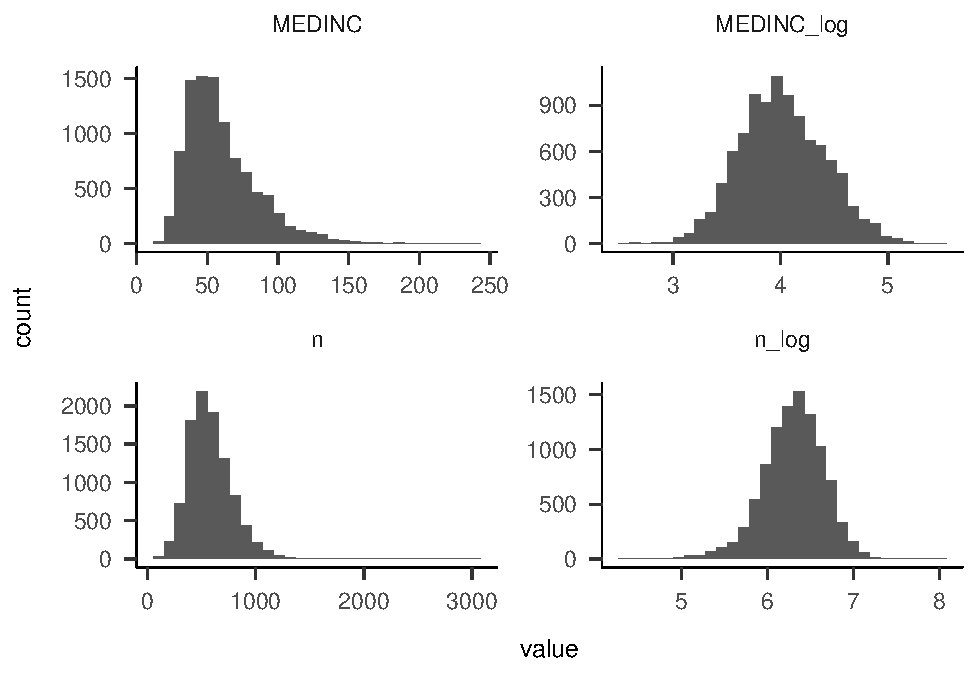
\includegraphics{GenSamp_Paper_Code_files/figure-latex/plot_dist1-1.pdf}
\caption{(\#fig:plot\_dist1)Comparison of covariate distributions and their log transformations.}
\end{figure}

\begin{Shaded}
\begin{Highlighting}[]
\NormalTok{plot_dist2}
\end{Highlighting}
\end{Shaded}

\begin{figure}
\centering
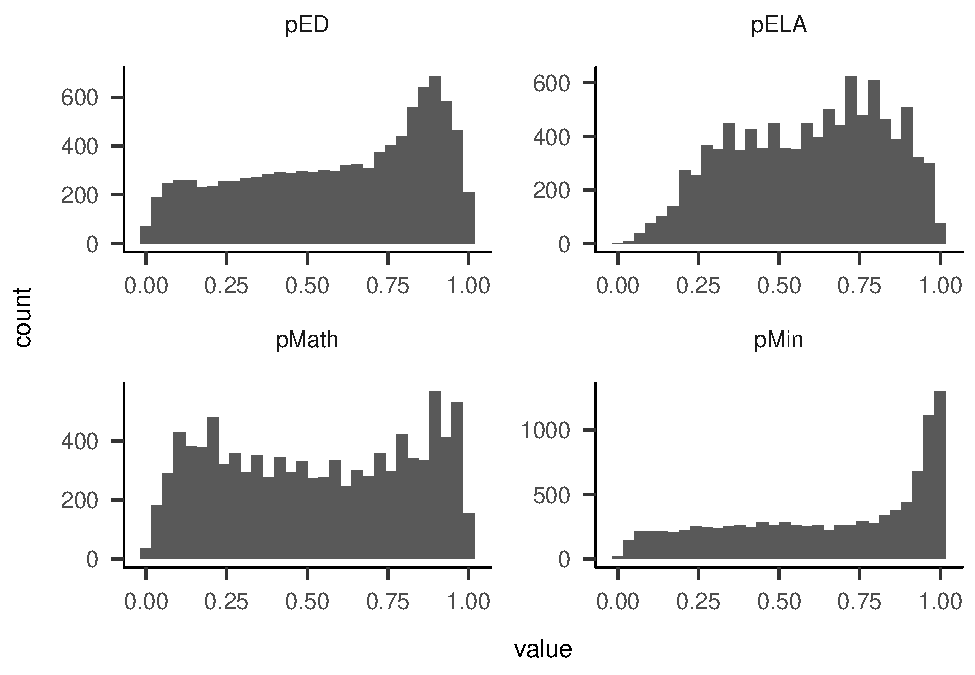
\includegraphics{GenSamp_Paper_Code_files/figure-latex/plot_dist2-1.pdf}
\caption{(\#fig:plot\_dist2)Distributions of the remaining continuous covariates.}
\end{figure}

\begin{Shaded}
\begin{Highlighting}[]
\KeywordTok{library}\NormalTok{(tidyverse)}
\KeywordTok{library}\NormalTok{(kableExtra)}

\KeywordTok{load}\NormalTok{(}\StringTok{"Data/RGM Vars.Rdata"}\NormalTok{)}

\NormalTok{tab_RGM_Pars <-}\StringTok{ }\NormalTok{schVals }\OperatorTok
\StringTok{  }\KeywordTok{select}\NormalTok{(Var, pars, RR) }\OperatorTok
\StringTok{  }\KeywordTok{mutate}\NormalTok{(}\DataTypeTok{RR =} \KeywordTok{paste}\NormalTok{(}\StringTok{"RR = "}\NormalTok{, RR}\OperatorTok{*}\DecValTok{100}\NormalTok{, }\StringTok{"%"}\NormalTok{, }\DataTypeTok{sep =} \StringTok{""}\NormalTok{),}
         \DataTypeTok{pars =} \KeywordTok{round}\NormalTok{(pars, }\DecValTok{2}\NormalTok{)) }\OperatorTok
\StringTok{  }\KeywordTok{spread}\NormalTok{(}\DataTypeTok{key =}\NormalTok{ RR, }\DataTypeTok{value =}\NormalTok{ pars) }

\CommentTok{# tab_RGM_Pars <- tab_RGM_Pars %>%}
\CommentTok{#   papaja::apa_table()}
\end{Highlighting}
\end{Shaded}

\begin{Shaded}
\begin{Highlighting}[]
\NormalTok{tab_RGM_Pars }\OperatorTok
\StringTok{  }\NormalTok{papaja}\OperatorTok{::}\KeywordTok{apa_table}\NormalTok{()}
\end{Highlighting}
\end{Shaded}

\begin{verbatim}
## 
## 
## \begin{table}[tbp]
## \begin{center}
## \begin{threeparttable}
## \caption{\label{tab:tab-RGM-Pars}}
## \begin{tabular}{llllllllll}
## \toprule
## Var & \multicolumn{1}{c}{RR = 10\%} & \multicolumn{1}{c}{RR = 20\%} & \multicolumn{1}{c}{RR = 30\%} & \multicolumn{1}{c}{RR = 40\%} & \multicolumn{1}{c}{RR = 50\%} & \multicolumn{1}{c}{RR = 60\%} & \multicolumn{1}{c}{RR = 70\%} & \multicolumn{1}{c}{RR = 80\%} & \multicolumn{1}{c}{RR = 90\%}\\
## \midrule
## Intercept & -2.99 & -1.83 & -1.09 & -0.27 & 0.77 & 1.52 & 4.61 & 3.62 & 7.49\\
## n & -0.17 & -0.16 & -0.20 & -0.20 & -0.21 & -0.24 & -0.21 & -0.42 & -0.40\\
## pED & 0.74 & 0.91 & 0.89 & 0.75 & 1.09 & 1.05 & 1.28 & 1.67 & 1.95\\
## pELA & 0.17 & 0.30 & 0.41 & -0.70 & 0.25 & -0.86 & 0.11 & -0.40 & 0.53\\
## pELL & -0.17 & -0.15 & -0.20 & -0.19 & -0.20 & -0.21 & 0.10 & -0.93 & -1.10\\
## pMath & 0.15 & 0.06 & -0.06 & 0.96 & 0.16 & 1.19 & 0.19 & 1.23 & 0.20\\
## pMin & -0.95 & -1.24 & -1.16 & -1.35 & -1.75 & -2.39 & -5.57 & -2.12 & -3.47\\
## Suburban & -0.18 & -0.07 & -0.28 & -0.64 & -0.50 & -0.19 & -0.51 & -0.02 & 1.40\\
## ToRu & 0.55 & 0.34 & 0.73 & 0.81 & 1.64 & 1.49 & 2.00 & 2.27 & 2.12\\
## Urban & -0.33 & -0.22 & -0.44 & -0.84 & -0.67 & -0.43 & -0.62 & -0.39 & -1.37\\
## \bottomrule
## \end{tabular}
## \end{threeparttable}
## \end{center}
## \end{table}
\end{verbatim}

\begin{Shaded}
\begin{Highlighting}[]
\KeywordTok{save.image}\NormalTok{(}\StringTok{"Paper Data/PaperData.rdata"}\NormalTok{)}
\end{Highlighting}
\end{Shaded}

\begin{Shaded}
\begin{Highlighting}[]
\KeywordTok{load}\NormalTok{(}\StringTok{"Paper Data/clusters-full-logs.rdata"}\NormalTok{)}
\NormalTok{ch_f <-}\StringTok{ }\NormalTok{chPlot}
\NormalTok{clusters_f <-}\StringTok{ }\NormalTok{clusters}

\NormalTok{ch_f}\OperatorTok{$}\NormalTok{subs <-}\StringTok{ "F"}

\CommentTok{# load("Paper Data/clusters-OV-logs.rdata")}
\CommentTok{# ch_ov <- chPlot}
\CommentTok{# clusters_ov <- clusters}
\CommentTok{# }
\CommentTok{# ch_ov$subs <- "OV"}
\CommentTok{# }
\CommentTok{# chPlot <- rbind(ch_f, ch_ov)}
\end{Highlighting}
\end{Shaded}

\begin{Shaded}
\begin{Highlighting}[]
\NormalTok{chPlot }\OperatorTok
\StringTok{  }\KeywordTok{gather}\NormalTok{(}\DataTypeTok{key =}\NormalTok{ method, }\DataTypeTok{value =}\NormalTok{ value, ch2) }\OperatorTok
\StringTok{  }\KeywordTok{ggplot}\NormalTok{(}\KeywordTok{aes}\NormalTok{(}\DataTypeTok{x =}\NormalTok{ k, }\DataTypeTok{y =}\NormalTok{ value)) }\OperatorTok{+}
\StringTok{  }\KeywordTok{geom_point}\NormalTok{() }\OperatorTok{+}
\StringTok{  }\KeywordTok{geom_line}\NormalTok{() }\OperatorTok{+}
\StringTok{  }\KeywordTok{theme_apa}\NormalTok{() }\OperatorTok{+}
\StringTok{  }\KeywordTok{scale_x_discrete}\NormalTok{(}\DataTypeTok{limits =} \KeywordTok{c}\NormalTok{(}\DecValTok{1}\OperatorTok{:}\NormalTok{K))}
\end{Highlighting}
\end{Shaded}

\begin{figure}
\centering
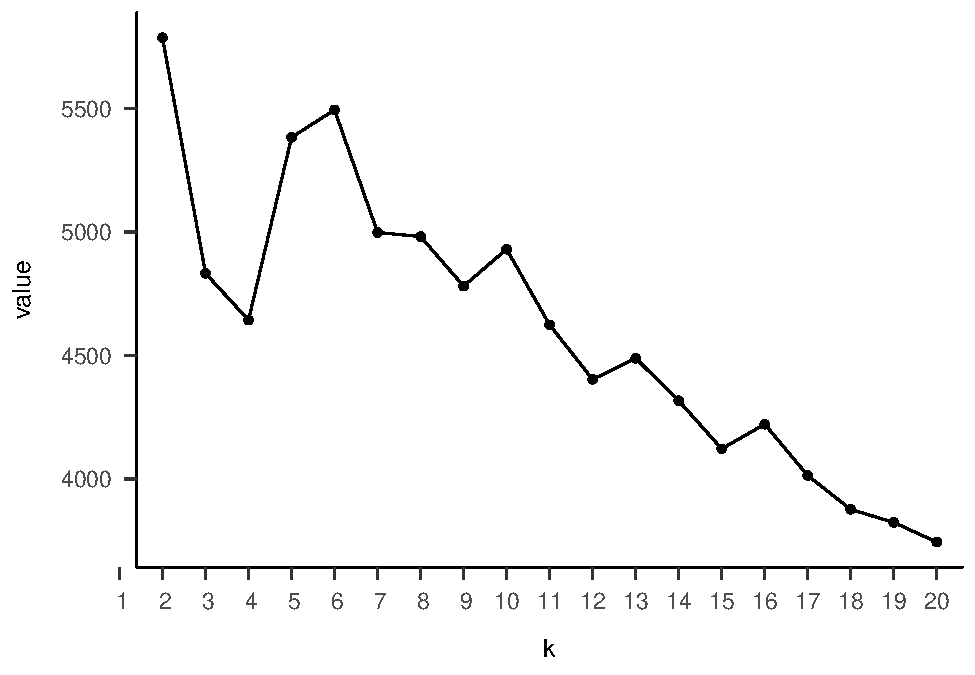
\includegraphics{GenSamp_Paper_Code_files/figure-latex/fig-ch-1.pdf}
\caption{\label{fig:fig-ch}Generalized Calinski-Harabasz index}
\end{figure}

\begin{Shaded}
\begin{Highlighting}[]
\CommentTok{# cls_ov <- bind_cols(lapply(clusters_ov, function(x) data.frame(x$cluster)))}
\NormalTok{cls_f <-}\StringTok{ }\KeywordTok{bind_cols}\NormalTok{(}\KeywordTok{lapply}\NormalTok{(clusters, }\ControlFlowTok{function}\NormalTok{(x) }\KeywordTok{data.frame}\NormalTok{(x}\OperatorTok{$}\NormalTok{cluster)))}

\CommentTok{# ratio_data <- rbind(data.frame(k = 1:K, subs = "F", vrat = unlist(lapply(clusters_f, function(x) x$betweenss / x$totss))),}
\CommentTok{#                     data.frame(k = 1:K, subs = "OV", vrat = unlist(lapply(clusters_ov, function(x) x$betweenss / x$totss))))}

\NormalTok{ratio_data <-}\StringTok{ }\KeywordTok{data.frame}\NormalTok{(}\DataTypeTok{k =} \DecValTok{1}\OperatorTok{:}\NormalTok{K, }\DataTypeTok{subs =} \StringTok{"F"}\NormalTok{, }\DataTypeTok{vrat =} \KeywordTok{unlist}\NormalTok{(}\KeywordTok{lapply}\NormalTok{(clusters, }\ControlFlowTok{function}\NormalTok{(x) x}\OperatorTok{$}\NormalTok{betweenss }\OperatorTok{/}\StringTok{ }\NormalTok{x}\OperatorTok{$}\NormalTok{totss)))}

\CommentTok{# levels(ratio_data$subs) <- c("Full", "Omitted Variable")}

\NormalTok{ratio_data }\OperatorTok
\StringTok{  }\CommentTok{# group_by(subs) %>%}
\StringTok{  }\KeywordTok{mutate}\NormalTok{(}\DataTypeTok{min80 =} \KeywordTok{sum}\NormalTok{(vrat }\OperatorTok{<}\StringTok{ }\FloatTok{.8}\NormalTok{) }\OperatorTok{+}\StringTok{ }\FloatTok{.5}\NormalTok{) }\OperatorTok
\StringTok{  }\CommentTok{# ungroup() %>%}
\StringTok{  }\KeywordTok{ggplot}\NormalTok{(}\KeywordTok{aes}\NormalTok{(}\DataTypeTok{x =}\NormalTok{ k, }\DataTypeTok{y =}\NormalTok{ vrat)) }\OperatorTok{+}
\StringTok{  }\KeywordTok{geom_point}\NormalTok{() }\OperatorTok{+}
\StringTok{  }\KeywordTok{labs}\NormalTok{(}\DataTypeTok{y =} \StringTok{"Between Cluster Variance"}\NormalTok{,}
       \DataTypeTok{x =} \StringTok{"Number of Strata (k)"}\NormalTok{) }\OperatorTok{+}
\StringTok{  }\KeywordTok{geom_line}\NormalTok{() }\OperatorTok{+}
\StringTok{  }\KeywordTok{geom_vline}\NormalTok{(}\KeywordTok{aes}\NormalTok{(}\DataTypeTok{xintercept =}\NormalTok{ min80), }\DataTypeTok{linetype =} \StringTok{"dashed"}\NormalTok{) }\OperatorTok{+}
\StringTok{  }\KeywordTok{theme_apa}\NormalTok{(}\DataTypeTok{box =}\NormalTok{ F) }\OperatorTok{+}
\StringTok{  }\KeywordTok{scale_x_discrete}\NormalTok{(}\DataTypeTok{limits =} \KeywordTok{c}\NormalTok{(}\DecValTok{1}\OperatorTok{:}\NormalTok{K)) }\OperatorTok{+}
\StringTok{  }\KeywordTok{scale_y_continuous}\NormalTok{(}\DataTypeTok{breaks =} \KeywordTok{seq}\NormalTok{(}\DecValTok{0}\NormalTok{, }\DecValTok{1}\NormalTok{, }\FloatTok{.1}\NormalTok{)) }\OperatorTok{+}\StringTok{ }
\StringTok{  }\CommentTok{# facet_grid(subs ~ ., , scales = "free") + }
\StringTok{  }\CommentTok{# facet_wrap( ~ subs, , scales = "free", ncol = 1) +}
\StringTok{  }\KeywordTok{theme}\NormalTok{(}\DataTypeTok{legend.position =} \StringTok{"none"}\NormalTok{,}
        \DataTypeTok{panel.spacing =} \KeywordTok{unit}\NormalTok{(}\DecValTok{2}\NormalTok{, }\StringTok{"lines"}\NormalTok{),}
        \DataTypeTok{text =} \KeywordTok{element_text}\NormalTok{(}\DataTypeTok{size=}\DecValTok{20}\NormalTok{),}
        \DataTypeTok{legend.title =} \KeywordTok{element_text}\NormalTok{(}\DataTypeTok{size=}\DecValTok{15}\NormalTok{))}
\end{Highlighting}
\end{Shaded}

\begin{figure}
\centering
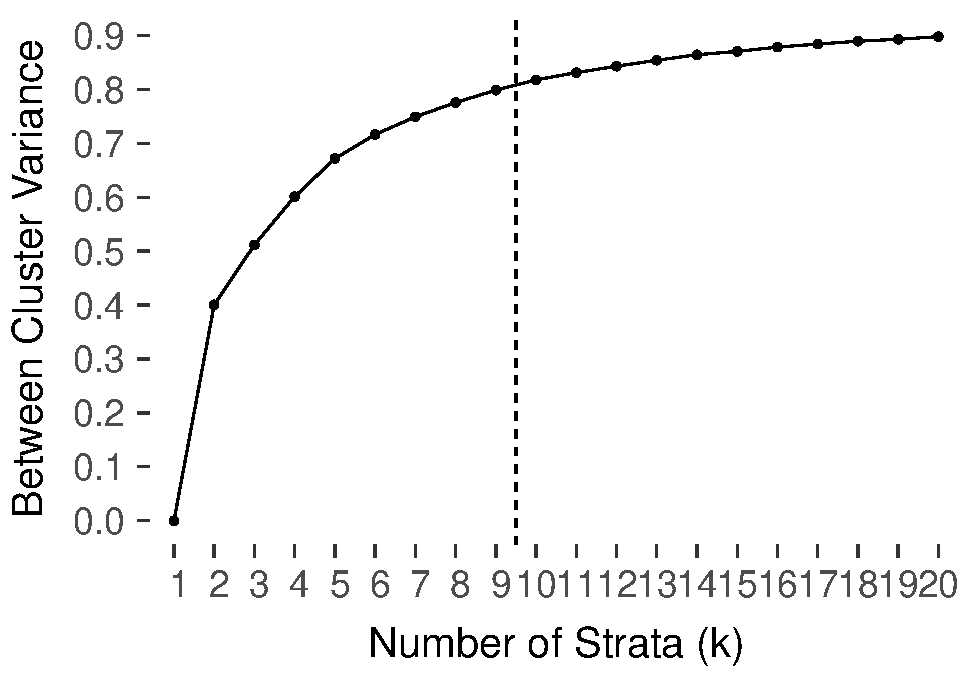
\includegraphics{GenSamp_Paper_Code_files/figure-latex/fig-ratio-1.pdf}
\caption{\label{fig:fig-ratio}Ratio of between cluster sum of squares to total cluster sum of squares}
\end{figure}

\begin{Shaded}
\begin{Highlighting}[]
\KeywordTok{ggsave}\NormalTok{(}\StringTok{"Figs/Elbow.jpg"}\NormalTok{, }\DataTypeTok{dpi =} \DecValTok{1000}\NormalTok{, }\DataTypeTok{width =} \DecValTok{10}\NormalTok{, }\DataTypeTok{height =} \FloatTok{8.5}\NormalTok{)}
\end{Highlighting}
\end{Shaded}

\begin{Shaded}
\begin{Highlighting}[]
\CommentTok{# names(cls_ov) <- names(cls_f) <- 1:K}
\KeywordTok{names}\NormalTok{(cls_f) <-}\StringTok{ }\DecValTok{1}\OperatorTok{:}\NormalTok{K}
\CommentTok{# cls_ov$subs <- "OV"}
\NormalTok{cls_f}\OperatorTok{$}\NormalTok{subs <-}\StringTok{ "F"}


\CommentTok{# rbind(cls_f, cls_ov) %>%}
\NormalTok{cls_f }\OperatorTok
\StringTok{  }\KeywordTok{gather}\NormalTok{(}\DataTypeTok{key =}\NormalTok{ k, }\DataTypeTok{value =}\NormalTok{ cluster, }\OperatorTok{-}\NormalTok{subs) }\OperatorTok
\StringTok{  }\KeywordTok{filter}\NormalTok{(k }\OperatorTok{>}\StringTok{ }\DecValTok{1}\NormalTok{) }\OperatorTok
\StringTok{  }\KeywordTok{mutate}\NormalTok{(}\DataTypeTok{k =} \KeywordTok{as.numeric}\NormalTok{(k)) }\OperatorTok
\StringTok{  }\KeywordTok{group_by}\NormalTok{(k, cluster, subs) }\OperatorTok
\StringTok{  }\KeywordTok{summarise}\NormalTok{(}\DataTypeTok{n =} \KeywordTok{n}\NormalTok{()) }\OperatorTok
\StringTok{  }\KeywordTok{group_by}\NormalTok{(k, subs) }\OperatorTok
\StringTok{  }\KeywordTok{mutate}\NormalTok{(}\DataTypeTok{sample =}\NormalTok{ (n }\OperatorTok{/}\StringTok{ }\KeywordTok{sum}\NormalTok{(n)) }\OperatorTok{*}\StringTok{ }\DecValTok{60}\NormalTok{) }\OperatorTok
\StringTok{  }\KeywordTok{ggplot}\NormalTok{(}\KeywordTok{aes}\NormalTok{(}\DataTypeTok{x =}\NormalTok{ k, }\DataTypeTok{y =}\NormalTok{ sample)) }\OperatorTok{+}
\StringTok{  }\KeywordTok{geom_point}\NormalTok{() }\OperatorTok{+}
\StringTok{  }\KeywordTok{theme_apa}\NormalTok{() }\OperatorTok{+}
\StringTok{  }\KeywordTok{labs}\NormalTok{(}\DataTypeTok{y =} \StringTok{"Allocated Sample Size"}\NormalTok{,}
       \DataTypeTok{x =} \StringTok{"Number of Strata (k)"}\NormalTok{) }\OperatorTok{+}
\StringTok{  }\KeywordTok{scale_x_discrete}\NormalTok{(}\DataTypeTok{limits =} \KeywordTok{c}\NormalTok{(}\DecValTok{1}\OperatorTok{:}\NormalTok{K)) }\OperatorTok{+}
\StringTok{  }\KeywordTok{scale_y_continuous}\NormalTok{(}\DataTypeTok{breaks =} \KeywordTok{seq}\NormalTok{(}\DecValTok{0}\NormalTok{, }\DecValTok{30}\NormalTok{, }\DecValTok{5}\NormalTok{)) }\OperatorTok{+}
\StringTok{  }\KeywordTok{stat_function}\NormalTok{(}\DataTypeTok{fun =} \ControlFlowTok{function}\NormalTok{(x) }\DecValTok{60}\OperatorTok{/}\NormalTok{x, }\DataTypeTok{geom =} \StringTok{"line"}\NormalTok{, }\DataTypeTok{linetype =} \StringTok{"dashed"}\NormalTok{) }\OperatorTok{+}
\StringTok{  }\CommentTok{# facet_grid(subs ~ .) +}
\StringTok{  }\KeywordTok{geom_hline}\NormalTok{(}\DataTypeTok{yintercept =} \DecValTok{5}\NormalTok{, }\DataTypeTok{linetype =} \StringTok{"dotted"}\NormalTok{)}
\end{Highlighting}
\end{Shaded}

\begin{figure}
\centering
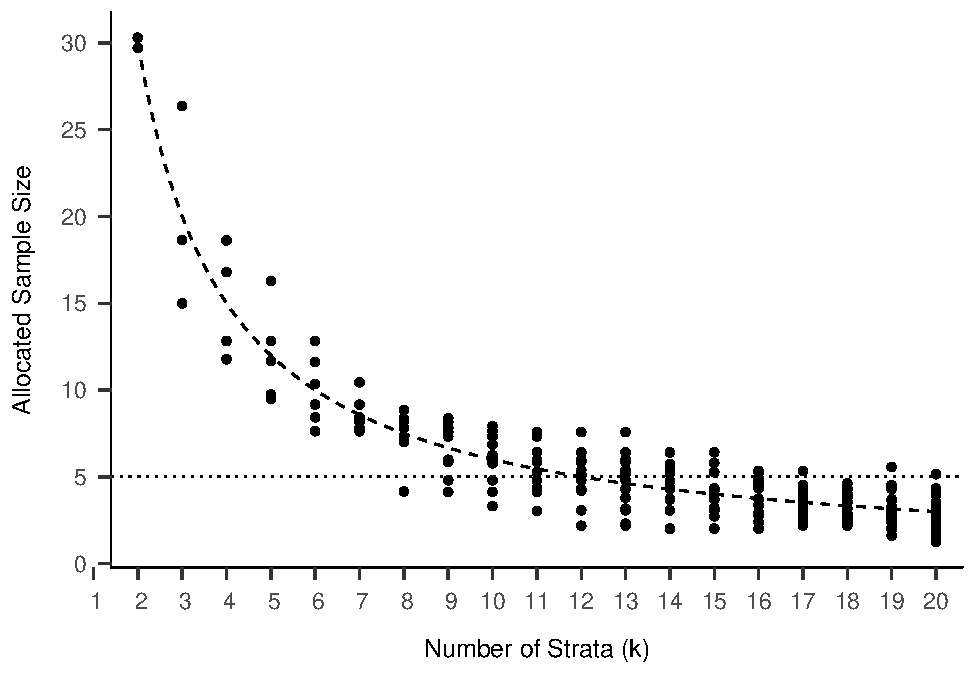
\includegraphics{GenSamp_Paper_Code_files/figure-latex/fig-k-size-1.pdf}
\caption{\label{fig:fig-k-size}Sampling requirements for each cluster}
\end{figure}

\begin{Shaded}
\begin{Highlighting}[]
\KeywordTok{save}\NormalTok{(chPlot, ratio_data, cls_f, }\DataTypeTok{file =} \StringTok{"Paper Data/Cluster data.rdata"}\NormalTok{)}
\end{Highlighting}
\end{Shaded}

\begin{Shaded}
\begin{Highlighting}[]
\CommentTok{# multiplot <- function(..., plotlist=NULL, file, cols=1, layout=NULL) \{}
\CommentTok{#   library(grid)}
\CommentTok{# }
\CommentTok{#   # Make a list from the ... arguments and plotlist}
\CommentTok{#   plots <- c(list(...), plotlist)}
\CommentTok{# }
\CommentTok{#   numPlots = length(plots)}
\CommentTok{# }
\CommentTok{#   # If layout is NULL, then use 'cols' to determine layout}
\CommentTok{#   if (is.null(layout)) \{}
\CommentTok{#     # Make the panel}
\CommentTok{#     # ncol: Number of columns of plots}
\CommentTok{#     # nrow: Number of rows needed, calculated from # of cols}
\CommentTok{#     layout <- matrix(seq(1, cols * ceiling(numPlots/cols)),}
\CommentTok{#                     ncol = cols, nrow = ceiling(numPlots/cols))}
\CommentTok{#   \}}
\CommentTok{# }
\CommentTok{#  if (numPlots==1) \{}
\CommentTok{#     print(plots[[1]])}
\CommentTok{# }
\CommentTok{#   \} else \{}
\CommentTok{#     # Set up the page}
\CommentTok{#     grid.newpage()}
\CommentTok{#     pushViewport(viewport(layout = grid.layout(nrow(layout), ncol(layout))))}
\CommentTok{# }
\CommentTok{#     # Make each plot, in the correct location}
\CommentTok{#     for (i in 1:numPlots) \{}
\CommentTok{#       # Get the i,j matrix positions of the regions that contain this subplot}
\CommentTok{#       matchidx <- as.data.frame(which(layout == i, arr.ind = TRUE))}
\CommentTok{# }
\CommentTok{#       print(plots[[i]], vp = viewport(layout.pos.row = matchidx$row,}
\CommentTok{#                                       layout.pos.col = matchidx$col))}
\CommentTok{#     \}}
\CommentTok{#   \}}
\CommentTok{# \}}
\CommentTok{# }
\CommentTok{# multiplot(ch_full, ratio_full, k_size_full, cols = 1)}
\end{Highlighting}
\end{Shaded}

\begingroup
\setlength{\parindent}{-0.5in}
\setlength{\leftskip}{0.5in}

\hypertarget{refs}{}

\endgroup


\end{document}
